\documentclass[hidelinks]{article}
\usepackage[francais]{babel}
\usepackage[utf8]{inputenc}
\usepackage[T1]{fontenc}
\usepackage{graphicx}
\usepackage{hyperref}
\usepackage{xcolor}
\usepackage{chngcntr}
\usepackage{float}
\counterwithin*{section}{part}
\usepackage[margin=2cm, bindingoffset=9mm]{geometry}

\title{%
	Projet d'électronique numérique \\
	\large{Visualisations musicales par VGA}}
\date\today
\author{
	\bsc{LESTANDI Nathan}
	\and
	\bsc{ECOCHARD Florent}
}

\begin{document}
    \pagenumbering{gobble}
    \maketitle
    \newpage
    \tableofcontents
    \pagenumbering{arabic}
    \newpage
    \part*{Introduction}
    \addcontentsline{toc}{part}{Introduction}
	A la suite de plusieurs séances de TPs d'approfondissement sur le langage de description VHDL dans l'environnement Vivado, nous avons eu à imaginer et mener à bien un projet étalé sur 7 semaines, en binôme. Le choix était assez libre et nous n'avions que peu de contrainte liées à l'énoncé du projet. Nous envisagions un sujet relié au son, car c'est un domaine qui nous intéresse tous les deux. Cependant, le traitement du son et notamment son acquisition et sa restitution sur la carte Artix 7 n'étant pas idéal, nous avons choisi de travailler sur un sujet à la croisée des chemins entre la synthèse vidéo et le traitement du son : un générateur de visualisations. Ce type de systèmes était très présent à une certaine époque sur les logiciels de lecture de fichiers sonores (Winamp, Windows Media Player, VLC etc.). De nos jours, c'est un domaine qui connaît un renouveau avec la pratique du VJing dans les performances de musique électronique.
	
	Cependant, étant donné notre niveau actuel de connaissances, du temps consacré aux projets et des limitations matérielles de la carte, les visualisations que nous avons réalisé sont très simplistes (voir le cahier des charges).
	
	De plus, Dans un souci d'efficacité et compte tenue de la complexité du sujet nous avons décidé d'utiliser le site Trello \cite{trello} afin de gérer la répartition des tâches et de fixer des deadlines. Ce site nous aura permis de suivre l'avancement de chacun en rendant régulièrement compte de notre travail, ainsi que de prendre des notes sur des éléments importants et des ressources.
	
    \section{Cahier des charges}
    Le cahier des charges général du projet impose une machine d'état ainsi qu'une interface utilisateur.
    
    
    \section{Architecture}
    \begin{figure}[h]
    \includegraphics[width=\textwidth, keepaspectratio=true]{VHDL_project_global_diagram1.png}
    \caption{\label{global} Schéma global du système}
    \end{figure}
    % Dans la figure~\ref{global} page~\pageref{global}, …
    \newpage
    \part{DSP : analyse du son}
    \section{Filtre passe-bas}
    \subsection{modélisation et dimension du filtre}
<<<<<<< 62f1e02b62a241022eeb430b22fb830f4cf2f62c
    Afin de réaliser un filtre passe-bas le moins encombrant possible et le plus facile à paramétrer, nous avons utilisé un filtre exponentielle du première ordre qui correspond à un filtre RC classique. En effet dans un RC la formule suivante apparait  : 
    \begin{center}
    	\begin{equation}
    	v_{in}(t)-v_{out}(t)=RC\frac{dv_{out}}{dt}
    	\end{equation}
    \end{center}
	Si on pose $v_{in}=x_n,\ v_{out}=y_n$ et $\frac{dv_{out}}{dt}=\frac{y_n-y_{n-1}}{\Delta_T}$ on obtient
=======
    Afin de réaliser un filtre passe-bas le moins encombrant possible et le plus facile à paramétrer, nous avons utilisé un filtre exponentiel du premier ordre qui s'écrit de la manière suivante: 
>>>>>>> corrections ortho
	\begin{center}
		\begin{equation}
			y(n)=(1-\epsilon)y(n-1)+x(n)\times\epsilon ,\; \epsilon=\frac{\Delta_T}{RC+\Delta_T} \ \in [0,1]
		\end{equation}
	\end{center}    
<<<<<<< 62f1e02b62a241022eeb430b22fb830f4cf2f62c
    Le filtre n'est composé que d'une seul variable : $\epsilon$, ça fréquence de coupure est définit par :
=======
    ce filtre correspond à un filtre RC,il ne possède qu'une seul variable : $\epsilon$, sa fréquence de coupure est définie par :
>>>>>>> corrections ortho
    \begin{center}
    	\begin{equation}
    	fc=\frac{-ln(1-\epsilon)}{2\pi}\times f_{fonctionnement}
    	\label{fc}
    	\end{equation}
    \end{center}    
<<<<<<< 62f1e02b62a241022eeb430b22fb830f4cf2f62c
    Cependant sous cette forme un déphasage est induit en haute fréquences. Pour remédier à ce problème,nous allons moyenner l'entrée avec l'échantillon précédent soit :
=======
    Cependant sous cette forme un déphasage est induit dans les haute fréquences. Pour remédier à ce problème, nous allons moyenner l'entrée avec l'échantillon précédent soit :
>>>>>>> corrections ortho
	\begin{center}
		\begin{equation}
			y(n)=(1-\epsilon)y(n-1)+\frac{(x(n)+x(n-1))\times\epsilon}{2}
			\label{formule_f}
		\end{equation}
	\end{center}  
    
    Sachant que nous travaillons sur une architecture numérique, il faut éviter les multiplication/divisions. Pour $\epsilon$ nous avons choisit de prendre des valeurs multiple de deux afin de limiter les opérations à des décalages.    
    Pour déterminer les $\epsilon$ de tous les filtres on prend comme fréquence de référence celle du \textit{enable} qui dépend du module de gestion de la carte SD, soit 44100Hz. Un $\epsilon$ de $2^{-4}=0.625$ permettra de couper à environ 450Hz tout en laissant les opération faites dans le filtre être de simple décalage.
    \begin{figure}[H]
    	\centering
    	 		\includegraphics[width=12cm,
    	 		keepaspectratio=true]{filtre_passe_bas.png}
    	\caption{\label{passe_bas}Schéma-bloc passe-bas}
    \end{figure}
<<<<<<< 62f1e02b62a241022eeb430b22fb830f4cf2f62c
   	On commence par synchronisé le circuit avec une bascule D, les autres bascules serviront à obtenir les valeurs n-1 de x et y nécessaires. les autres calculs seront fais dans des processus implicite.\\
   	Dans l'équation \ref{fc} on identifie $f_{fonctionnement}$. Dans notre modélisation du filtre, sans un signal enable, ce serait la clock qui fournirait cette fréquence. Hors on scrute aussi le signal enable pour activer les bascules, on a donc :\\$f_{fonctionnement}=f_{enable}=44100Khz$, valeur qui est fournit par le module SD.
=======
   	On commence par synchroniser le circuit avec une bascule D. Les autres serviront à obtenir les valeurs n-1 nécessaires aux calculs. les autres calculs seront faits dans des processus implicites.\\ % à réécrire
   	
   	Dans l'équation \ref{formule_f} on identifie $f_{fonctionnement}$. Dans notre modélisation du filtre, sans un signal enable, ce serait l'horloge qui fournirait cette fréquence. Or, on scrute aussi le signal enable pour activer les bascules. On a donc :\\$f_{fonctionnement}=f_{enable}=44100Khz$, valeur qui est fournie par le module SD.
>>>>>>> corrections ortho
   	
    \subsection{simulation}
	Nous avons décidé de préciser la simulation du passe-bas car c'est le bloc de base des autres filtres. Il es donc indispensable de comprendre son fonctionnement.

    
    \subsubsection{test bench}
    Pour simuler ce bloc, nous avons créé un «testbench» basique. Pour rédiger la trame principale nous avons utilisé le site internet Lapinoo\cite{lapinoo}. Nous avons ensuite complété le testbench de manière a tester le signal d'entrée , le reset, le signal enable et la sortie. Pour cela nous avons imposé des valeurs en entrée, puis nous avons confronté les résultat aux valeurs théoriques calculées à partir de la formule (\ref{formule_f}).\\
    
    \subsubsection{Simulation et interprétation}
    Voici une capture de la simulation obtenue :
    \begin{figure}[h]
    	\centering
    	\includegraphics[width=15cm, keepaspectratio=true]{simu_pb_1.PNG}
    	\caption{schéma bloc passe-bas}
	\end{figure}
	Sur celle-ci nous pouvons observer plusieurs choses, mais nous allons d'abords scruté les effets du reset et d'enable pour voir si ils répondent aux attentes.
	
	Le signal reset est testé dans la partie la plus à droite délimité par le carré, on voit qu'il remet bien à 0 toute les sorties.
    
    
    Le signal enable est lui testé dans le carré jaune, on voit que lorsqu'il est à zéro, le système ne varie pas. Ce qui est l'effet escompté puisque ce signal correspond à l'envoie en entrée d'un échantillon audio. Sans échantillon le filtre ne doit pas fonctionner.
    
    Vérifions maintenant la fonction effectué par le bloc, pour cela nous allons nous concentrer sur les 2 coups d'horloge dans le carré vert. Pour savoir la correspondance des signaux, se refferé à la figure \ref{passe_bas}.
    On observe bien sur le premier coup d'horloge encadré que x-sum-par32 correspond bien à ${\frac{x(n)+x(n-1)}{2^{-5}}}$, avec les valeurs binaire, un décalage de 5 vers la droite est bien effectué. De même y-diff est bien correspond à $y(n-1)\times(1-\epsilon$). La sortie est bien égale à xy qui est la somme de x-sum-par32 et y-diff. Les décalages sont bien effectué entre deux coups d'horloge, ce qu'on peut vérifier en comparant avec le deuxième coup d'horloge dans le cadre vert: x-1 et y-1 sont bien x(n-1) et y(n-1).
    %image
	
    \section{Filtre passe-haut}
    Pour le passe-haut nous allons utiliser un principe instinctif suivant lequel, modéliser un passe-haut revient à soustraire au signal d'entrée ça valeur filtré dans un passe-bas soit :
    \begin{figure}[h]
    	\centering
    	\includegraphics[width=12cm, keepaspectratio=true]{passe-haut-simplifie.png}
    	\caption{schéma bloc passe-haut}
    \end{figure}

	On utilise une bascule D sur entrée-x afin de synchronisé celle-ci avec le bloc passe-bas. Nous avons fixé $\epsilon$=$2^{-1}$ de manière à avoir une fréquence de coupure plus haute que le passe-bas soit environ 5Khz. Pour ce faire nous avons utilisé un generic : n qui correspond à la puissance d'  $\epsilon$ dans le filtre passe-bas.  \\
	Nous vérifierons que le bloc à une réponse impulsionnelle correspondant à un passe- haut dans la figure \cite{sim_dsp}
	\newpage 

    \section{Filtre passe-bande}
	Pour créer le passe-bande, nous avons mis en série le passe haut et le passe-bas soit:
	\begin{figure}[h]
		\centering
		\includegraphics[width=12cm, keepaspectratio=true]{passe_bande_simpli.png}
		\caption{schéma bloc passe-bande}
	\end{figure}

	On utilise les blocs précédents en branchant la sortie directement sur celle du passe haut
	on garde ici le même epsilon dans le passe bas que dans sa version original, de même pour le passe haut, de cette manière on couvre l'intégralité du spectre du signal.

    \section{Bloc DSP}
    Le bloc DSP regroupe les parties précédentes , il envoie en continue les sortie des 3 filtres aux étages de visualisation.
    
	\begin{figure}[h]
		\centering
		\includegraphics[width=10cm, keepaspectratio=true]{DSP.png}
		\caption{schéma DSP}
	\end{figure}
	Afin de prouver le bon fonctionnement nous avons tester la réponse impulsionnelle de l'ensemble du bloc DSP. Pour ce faire nous avons fixé l'entrée à une valeur, ici 32768 (en binaire 1000000000000000) et nous avons regarder la sortie des filtres de manière analogique( waveform style -> analog) et on a:
	
	\begin{figure}[H]
		\centering
		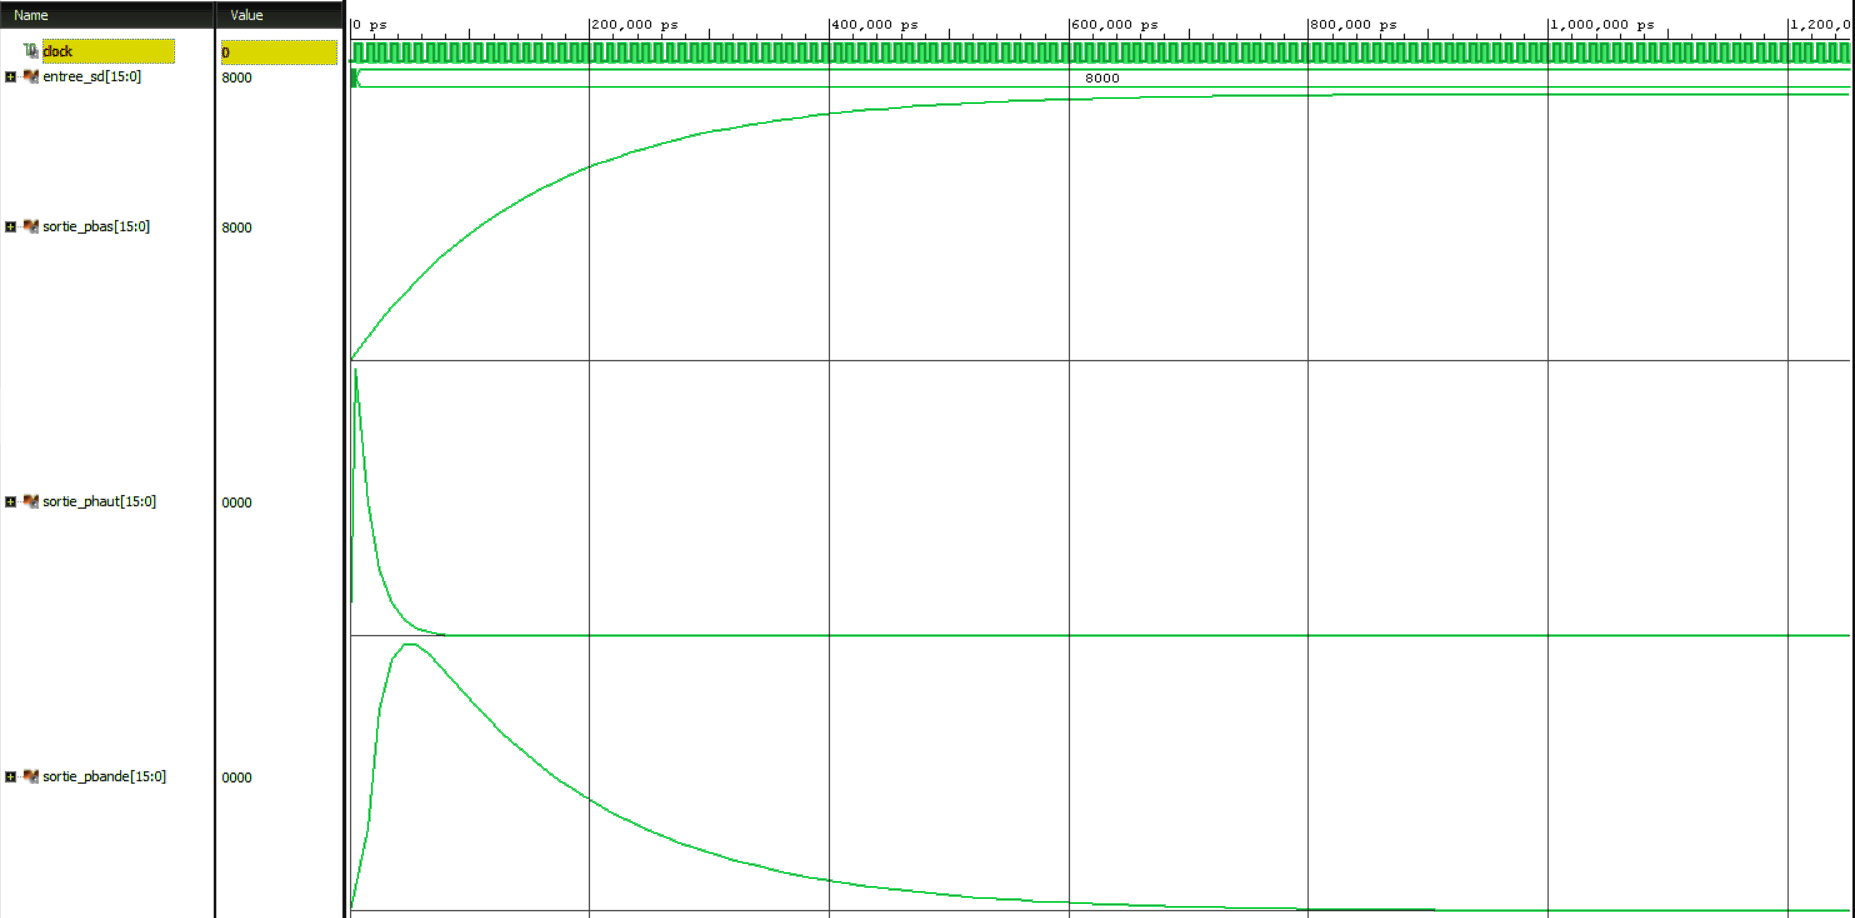
\includegraphics[width=10cm, keepaspectratio=true]{DSP_impulsion.PNG}
		\caption{réponse impulsionnelle bloc DSP}
	\end{figure}

	La sortie du passe-bas tend bien vers la valeur du signal lorsque celui-ci reste longtemps en entrée et inversement pour le passe-haut, il coupe lorsque le signal reste longtemps identique. Le passe bande est bien un compromis des deux en filtrant lorsque la fréquence est trop haute ou trop basse.\\
	Nous avons mesuré les fréquences de coupure pour chacun de ces filtres en prenant pour fréquence de référence celle de la carte soit 100Mhz, on a alors $\tau_{p-b}$=150ns pour le passe-bas et $\tau_{p-h}$=15 ns pour le passe haut d'après la formule \ref{formule_f}. Nous avons bien des valeurs constantes en sortie des filtres regardant leur réponses qui est constante à 5 $\tau$ (75ns et 750ns).
	\newpage

    \part{Visualisations, affichage}
    %\subsection{}
    %\paragraph{}    
    \section{L'"oscilloscope"}
    %\subsection{}
    %\paragraph{}    
    \section{Le "spectrogramme"}
    %\subsection{}
    %\paragraph{}    
    \section{Le bargraph}
    %\subsection{}
    %\paragraph{}
    \part*{Bilan}
    \addcontentsline{toc}{part}{Bilan}
  
\newpage
\bibliographystyle{plain} % Le style est mis entre accolades.
\bibliography{bibli} % mon fichier de base de données s'appelle bibli.bib
https://tomroelandts.com/articles/low-pass-single-pole-iir-filter
https://fiiir.com/
http://www.dspguide.com/ch19/2.htm
\addcontentsline{toc}{section}{Bibliographie}


\end{document}